% 第 19 题圆锥图：按固定源内容流矢量层精确值复刻（1 pt → 0.03515 cm）。
% 原点取底面圆心 O（源页 (693.454, 395.647) pt），y 向上。
% 底面为透视缩扁的椭圆：半长轴 68.0346、半短轴 25.7095（PO/OA = 2.00000 与题设严格一致）。
% 实线 4 条：母线 PC、母线 PA/PB（照源画作椭圆切线，落点 (±66.842, +4.847) 不在 A/B 上）、
% 近侧半弧（下，参数角 170°→350°）；虚线 6 条：轴线 PO、直径 AB、弦 AC、
% 半径 OC 与 OE、远侧半弧（上，参数角 10°→170°）。虚线节距照源 [on 2.989 off 2.989]。
% 源内瑕疵照录：C 位于参数角 249.30°（题设「半圆弧 AB 的中点」应为 270.000°、偏 20.70°）；
% E 严格为弧 C→B 中点（304.63°，与题设一致）；母线端点比 A/B 高 4.847 pt、各内收 1.193 pt。
% 全图无点记号、无箭头、无填充；六个标签照源文本原点（基线左端）定位。
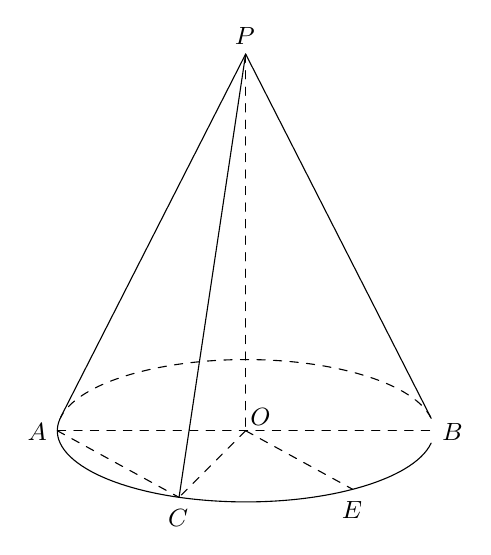
\begin{tikzpicture}[line cap=round,line join=round,font=\small,x=0.03515cm,y=0.03515cm]
% ===== 椭圆底（两半弧照源分开绘制：远侧虚线 / 近侧实线）=====
\draw[dash pattern=on 2.989pt off 2.989pt, line width=0.398bp] (67.0001,4.4643) arc [start angle=10, end angle=170, x radius=68.0346, y radius=25.7095];   % 远侧半弧（上，虚线）
\draw[line width=0.398bp] (-66.9989,4.4643) arc [start angle=170, end angle=350, x radius=68.0346, y radius=25.7095];   % 近侧半弧（下，实线）
% ===== 实线 3 条（母线；PA/PB 照源为切线画法）=====
\draw[line width=0.398bp] (0,136.069)--(-24.067,-24.0669);   % P–C
\draw[line width=0.398bp] (0,136.069)--(-66.842,4.8471);   % P–左切点（PA）
\draw[line width=0.398bp] (0,136.069)--(66.842,4.8471);   % P–右切点（PB）
% ===== 虚线 5 条（轴线/底面辅助线）=====
\draw[dash pattern=on 2.989pt off 2.989pt, line width=0.398bp] (0,136.069)--(0,0);   % P–O（轴线）
\draw[dash pattern=on 2.989pt off 2.989pt, line width=0.398bp] (-68.0346,0)--(68.0344,0);   % A–B（直径）
\draw[dash pattern=on 2.989pt off 2.989pt, line width=0.398bp] (-68.0346,0)--(-24.067,-24.0669);   % A–C（弦）
\draw[dash pattern=on 2.989pt off 2.989pt, line width=0.398bp] (0,0)--(-24.067,-24.0669);   % O–C（半径）
\draw[dash pattern=on 2.989pt off 2.989pt, line width=0.398bp] (0,0)--(38.695,-21.176);   % O–E（半径）
% ===== 标注（照源文本原点＝基线左端，显式坐标）=====
\node[anchor=base west,inner sep=0] at (-4.1,139.456) {\(P\)};
\node[anchor=base west,inner sep=0] at (1.485,2.048) {\(O\)};
\node[anchor=base west,inner sep=0] at (-78.946,-3.588) {\(A\)};
\node[anchor=base west,inner sep=0] at (70.763,-3.588) {\(B\)};
\node[anchor=base west,inner sep=0] at (-28.195,-34.629) {\(C\)};
\node[anchor=base west,inner sep=0] at (34.516,-31.737) {\(E\)};
\end{tikzpicture}
